%%
%
% ARQUIVO: cap-01.tex
%
% VERSÃO: 1.0
% DATA: Maio de 2016
% AUTOR: Coordenação de Trabalhos Especiais SE/8
% 
%  Arquivo tex de exemplo de capítulo do documento de Projeto de Fim de Curso.
%
% ---
% DETALHES
%  a. todo capítulo deve começar com \chapter{•}
%  b. usar comando \noindent logo após \chapter{•}
%  c. citações para referências podem ser
%       i. \citet{•} para citações diretas (p. ex. 'Segundo Autor (2015)...'
%       ii. \citep{•} para citações indiretas (p. ex. '... (AUTOR, 2015)...'
%  d. notas de rodapé devem usar dois comandos
%       i. \footnotemark para indicar a marca da nota no texto
%       ii. \footnotetext{•}, na sequência, para indicar o texto da nota de rodapé
%  e. figuras devem seguir o exemplo
%       i. devem ficar no diretório /img e devem ser no formato EPS
%  f. tabelas devem seguir o exemplo
%  g. figuras e tabelas podem ser colocadas em orientação landscape
%       i. figuras: usar \begin{sidewaysfigure} ... \end{sidewaysfigure}
%                   em vez de \begin{figure} ... \end{figure}
%       ii. tabelas: usar \begin{sidewaystable} ... \end{sidewaystable}
%                    em vez de \begin{table} ... \end{table}
%  h. toda figura e tabela deve ser referenciada ao longo do texto com \ref{•}
% ---
%%

\chapter{introdução}
\noindent
A tarefa de verificar a presença dos alunos é uma constante na sala de aula. Todo início de aula é marcado por esse processo. Ele é extremamente importante para a vida acadêmica dos alunos, uma vez que a falta acarreta na perda de pontos, o que pode levar, em casos extremos, a exclusão do aluno.
\section{Contextualização do Tema}
Por ser uma instituição de ensino com aulas presenciais e cumprir as exigências do Ministério da Educação, o Instituto Militar de Engenharia, exige, em seu regulamento que trata sobre a frequência escolar \citep{NICFA}, que seus alunos mantenham um alto índice de presença nas aulas ao longo do período escolar. De modo a verificar esse objetivo, existe um sistema de apuração de faltas que consiste na entrega da papeleta de faltas, uma papeleta preenchida a caneta contendo a identificação de todo e qualquer estudante ausente em cada um dos tempos de aula do dia. O preenchimento das papeletas é de responsabilidade de um aluno escalado,  o qual, na seção de Engenharia da Computação, faz tal tarefa em três vias: duas vias entregues à Seção de Ensino e uma via entregue ao Corpo de Alunos. Além disso, os professores têm de assinar a papeleta, em suas 2 vias. As Seções de Ensino fazem o lançamento das faltas no sistema acadêmico do IME e recebem as justificativas de faltas dos alunos da reserva. O CA recebe as justificativas das faltas dos alunos da ativa e abre processo de apuração de transgressão disciplinar quando ocorre uma falta não justificada.  

\section{Motivação}
Diante do exposto, podemos identificar uma série de problemas nesse processo: a manutenção de arquivos do mesmo documento,  sendo um em cada seção; lentidão de consulta ao arquivo, devido ao grande acúmulo de papel; possibilidade de perda de papeletas, comprometendo a apuração das faltas; maior probabilidade de conter informações imprecisas ou incorretas, como erros de lançamento; e aumento do fluxo de documentos em cada seção. Outrossim, o processo depende da interação de diversos atores, o que aumenta a probabilidade de uma falha.

Além disso, a apuração da falta cabe ao chefe de turma, segundo as normas que especificam as funções e responsabilidades \citep{NEFSE}. Dessa maneira, cabe ao aluno a verificação de presença dos seus colegas e a sua própria, fugindo assim da idealidade,  já que acumula os papeis de fiscalizado e fiscalizador.
%já que se coloca um fiscalizado na posição de fiscalizador.

É importante ressaltar que \citep{NICFA} dispõem no seguinte sentido: "o acúmulo superior a 120 pontos perdidos, em faltas, resulta na reprovação, desligamento e exclusão do aluno, impedindo-o de concluir seu curso no IME". Assim sendo, fica evidente a necessidade de um sistema ágil e preciso, que simplifique a apuração das faltas pelos responsáveis.

\section{Objetivo}
Considerando a motivação apresentada na seção anterior, o objetivo desse trabalho é desenvolver um sistema informatizado capaz de automatizar o processo de apuração e registro de faltas. Para tanto, será feito o uso de reconhecimento facial e de tecnologia de desenvolvimento móvel como principais ferramentas, estando também presentes no sistema uma conexão cliente-servidor e um banco de dados.

A estrutura geral do sistema, como se pode ver na Figura \ref{fig:figura1}, consiste na interação entre dois dispositivos, sendo um cliente e um servidor. O primeiro será um dispositivo móvel Android, cuja tarefa é enviar ao servidor uma foto dos alunos presentes no início de cada tempo de aula, bem como as informações sobre a turma e a aula. O segundo dispositivo será um servidor que terá como entrada as informações enviadas pelo cliente e um boleto contendo as faltas como saída. As faltas serão apuradas por meio de algoritmos de reconhecimento facial, os quais irão reconhecer as faces contidas na foto recebida, marcando como presentes os alunos reconhecidos e salvando essa informação no banco de dados. Dessa forma, o registro de frequências ficará armazenado nesse banco de dados, o qual pode ser consultado sempre que for necessário, eliminando a necessidade do uso de papel. Como maneira corretiva para eventuais erros, o professor e o aluno podem atuar. A arquitetura será explicada com mais detalhes em um capítulo próprio.
\section{Justificativa}
Fica evidente, então, que a retirada de falta é um processo muito importante na vida acadêmica do aluno, podendo inclusive acarretar, nos casos mais extremos, em sua reprovação. Dada a importância desse processo, o produto deve ser tão fiel quanto possível à realidade, apresentando de maneira correta e precisa os discentes presentes e ausentes naquele tempo de aula.

Com a proposta de sistema ora feita, os erros causados pelo fator humano e o retrabalho mencionados na motivação são mitigados. Dessa forma, consegue-se um processo mais eficiente com produtos mais fidedignos. 

\section{Metodologia}
A metodologia adotada para alcançar o objetivo proposto para este trabalho se divide em: fundamentação teórica, projeto e implementação de prova de conceito. Visando a correta implementação do sistema proposto, a fundamentação teórica faz-se necessária para a correta compreensão de conceitos como reconhecimento e detecção facial, os quais se constituem como o cerne da atividade proposta por esse trabalho. O projeto envolve a modelagem e o planejamento de desenvolvimento do sistema.  Na fase de implementação de prova de conceito ocorrerá a realização de testes a fim de verificar a acurácia na verificação de faltas e o comportamento do sistema como um todo. 

%\begin{itemize}
%\item \textit{Fundamentação Teórica:} Para a correta implementação do sistema proposto, faz-se necessário a correta compreensão de conceitos como aprendizagem de máquina, reconhecimento e detecção facial, além de algoritmos empregados nesses processos. Cabe também destacar a importância do tipo de comunicação entre o cliente e o servidor.
%\item \textit{Projeto:} Nessa fase se dá a modelagem do projeto. Será definida a estrutura, os entregáveis previstos e o cronograma do trabalho.
%\item \textit{Implementação de Prova de Conceito:} Nessa fase ocorrerá a implementação de testes a fim de verificar a acurácia na verificação de faltas e o comportamento do sistema como um todo. 
%\end{itemize}


\begin{figure}[!ht]
	\centering
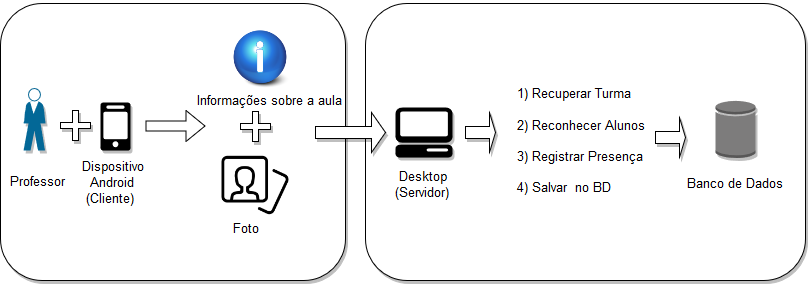
\includegraphics[width=1.0\textwidth]{img/diagramaintro.png}   
	\caption{Estrutura do Sistema}
	\label{fig:figura1}
\end{figure}

\section{Estrutura}
Este trabalho será organizado de acordo com o seguinte formato: O capítulo 1 traz uma breve introdução e contextualização do tema. o capítulo 2 contém os conceitos básicos relacionados à detecção e reconhecimento facial; o capítulo 3 trata da modelagem do sistema; o capítulo 4 aborda a construção do módulo servidor, esse módulo contempla o reconhecimento facial; o capítulo 5 trata do módulo \textit{mobile}, mostrando o aplicativo desenvolvido e o programa que executado no servidor é responsável por receber a fotografia e as informações enviadas pelo professor, como seu desenvolvimento estava intimamente ligado com o aplicativo, optou-se por descrevê-lo nesse capítulo; o capítulo 6 descreve o módulo BD, e é responsável pela criação do esquema no banco de dados, aborda-se ainda a conexão do módulo servidor com o banco de dados, além de se abordar a interface web (servidor web)  para visualização e alteração das papeletas; o capítulo 7 faz a Análise crítica do sistema, e por fim, o capítulo 8 aborda a  conclusão do projeto.
%\begin{itemize}
%\item \textit{Capítulo 2:} Será realizada a discussão sobre os conceitos básicos relacionados a detecção e reconhecimento facial.
%\item \textit{capítulo 3:} Define-se a modelagem do sistema, dividindo-o em módulos. 
%\item \textit{Capítulo 4:} %Novos capitulos pra VC
%\item \textit{Capítulo 5:} %Novos capitulos pra VC
%\item \textit{Capítulo 6:} descrição e explicação do planejamento do projeto.
%\item \textit{Capítulo 7:} expõem a conclusão parcial do projeto.


%\end{itemize}



